\documentclass[Orbiter User Manual.tex]{subfiles} 
\begin{document}

\section{Flight checklists and challenges}
This section contains point-by-point checklists for some complete flights. The scenarios for the checklist flights can be found under the \textit{Checklists} folder in the Orbiter Launchpad dialog. While performing these missions, you may want to save regularly (\Ctrl\keystroke{S}), so you can pick up from a previous state if necessary.\\
The checklists for these flights can also be accessed during the simulation by calling up help (\Alt\keystroke{F1}) and clicking the \textit{Scenario} button in the help window. Other scenarios may also provide inline help.\\
The flight challenges (under the \textit{Challenges} folder) consist of a set of missions that demand some skills in planning and navigation. You get a score depending on how well you completed the mission within the specified parameters.

\subsection{Checklist mission 1: Delta-glider to ISS}
In this mission we launch the Delta-glider spaceplane into orbit from runway 33 of the Shuttle Landing Facility (SLF) at Kennedy Space Center, and perform a rendezvous and docking manoeuvre with the International Space Station.

\begin{itemize}
\item Start Orbiter with the \textit{Checklists/DG to ISS} scenario. Your glider is on the runway, ready for take-off.
\item You may need to scroll the instrument panel down a bit (\UArrow$_{Cur}$) to see the runway in front of you. Make sure you can still see the top half of the panel with the MFD screens.
%TODO add section link
\item Your launch is scheduled for MJD = 51983.6308 (the \textit{Modified Julian Date}, or \textit{MJD}, is Orbiter's universal time reference, and is shown in the top right corner of the screen). This leaves plenty of time to get used to the instrumentation. If you are not yet familiar with the DG's panel layout, check TODO. For details on MFD modes see TODO.
\item The left MFD instrument is in \textit{Surface} mode and shows velocity and altitude data during flight.
\item The right MFD is in \textit{Map} mode and shows your current location at KSC as a green cross, labelled GL-01. The orbital plane of the ISS is shown as a yellow curve. As time progresses and Earth rotates under the space station's orbit plane, the curve will shift across the map.
%TODO symbol
\item To fast-forward to your launch window, press \keystroke{T}. (Each time you press \keystroke{T}, time speeds up by a factor of 10.) As you approach launch time, switch back to real-time by pressing \keystroke{R} until the TODO indicator in the top right corner of the screen disappears.
\item Launch when the space station's orbital plane crosses your landing site (to zoom into the MFD map display, press the ZM+ button (\Shift\keystroke{Z}).
\item Engage main engines at 100\% thrust: Press and hold \keystroke{+}$_{Num}$, then \Ctrl to lock thrust setting. You may also use the sliders in the instrument panel or the throttle control on your joystick to operate the main engines.
\item At ground speed 150 m/s (Surface MFD or HUD readout), pull the stick (or press \keystroke{2}$_{Num}$) to rotate.
\item Climb at 10° and retract the landing gear (\keystroke{G}).
\item Turn right towards a heading of 140°.
\item Pitch up steeply to 70°. We want to climb quickly out of the dense lower part of the atmosphere to avoid friction losses and excessive hull heating as we build up speed.
\item At about 30 km altitude the glider will start to drop its nose due to decreasing atmospheric pressure, even while pulling back on the stick. Activate the RCS (Reaction Control System) by clicking the right part of the \textit{RCS Mode} selector dial (on the right side of the instrument panel) or by pressing \keystroke{/}$_{Num}$. You are now controlling your craft with attitude thrusters.
\item Pitch down to about 20°. At this point we need to start gaining tangential velocity to achieve orbit. Your flight path indicator (the $\oplus$ symbol in the HUD) should stay above 0°.
\item Switch the right MFD to \textit{Orbit} mode (\Shift\keystroke{F1}+\Shift\keystroke{O}). Select the ship's orbit as reference plane (\Shift\keystroke{P}) and select the ISS as target (\Shift\keystroke{T}, \Enter, 'ISS', \Enter).
\item Continue at 100\% main thrust and maintain your heading. Adjust pitch angle so that the flight path vector remains slightly above 0°. As the horizontal component of your velocity vector increases, the orbit trajectory (green curve in the Orbit MFD) starts growing.
\item Cut engines when the apogee radius (highest point of the orbit) reaches 6.731M (the ApR entry in the left column of the Orbit MFD). This corresponds to an altitude of 360 km.
\item Switch to Orbit HUD mode (\keystroke{H}+\keystroke{H}, or press the HUD button in the Orbit MFD).
\item At the moment we are on a ballistic flight path that would eventually bring us back to the surface. To enter orbit we need to perform a further burn (orbit insertion burn) at the apex of the trajectory. Wait until you reach apogee (the remaining time is shown as ApT in the Orbit MFD). This could take a while, so you may want to time-accelerate.
\item At apogee, press the PRO-G button (shortcut: \keystroke{[}) to activate the \textit{prograde} attitude mode. One the velocity marker ($\oplus$) is centred in the HUD, engage main thrusters until orbit eccentricity (Ecc value in Orbit MFD) reaches a minimum, and perigee radius (PeR) approximately equals ApR. This will require only a short burn!
\item Switch the left MFD to \textit{Plane Alignment} mode (\Shift\keystroke{F1}+\Shift\keystroke{A}). Select ISS as target (\Shift\keystroke{T}, \Enter, 'ISS', \Enter).
\item Your orbital plane should already roughly match that of the ISS (RInc $\leq$ 5°), thanks to the chosen launch time and azimuth. We now need to fine-adjust the plane.
\item As your ship (P) approaches the intersection point (\textit{node}) with the target plane (AN or DN): Rotate the ship perpendicular to your current orbital plane (90° on the Orbit HUD inclination ladder). If you are approaching the \textit{ascending node} (AN), turn \textit{orbit-antinormal} (the NML- attitude mode button, shortcut \keystroke{'}). If you are approaching the \textit{descending node} (DN), turn \textit{orbit-normal} (the NML+ attitude mode button, shortcut \keystroke{;}).
\item As soon at the \textit{time-to-burn} (TtB) counter for the node has reached zero and the [BURN] indicator appears, fire the main engines at 100\% for the indicated \textit{burn time} (BT). The relative inclination (RInc) between the current and target planes should now decrease.
\item Cut engines when the BT counter reaches zero and the [BURN] indicator is turned off. If the planes were not sufficiently aligned in this manoeuvre (RInc within $\sim$0.5°), repeat the process at the next node crossing.
\item Once the planes are aligned, the next step is intersecting the ISS. Switch to \textit{Sync Orbit} MFD mode (\Shift\keystroke{F1}+\Shift\keystroke{Y}). Select ISS as target (\Shift\keystroke{T}, \Enter, 'ISS', \Enter), and switch the reference point to \textit{Intersect 1} or \textit{Intersect 2} (\Shift\keystroke{M}). If the orbits don't intersect, select \textit{Sh periapsis} instead.
\item The two columns on the right of the MFD display show the times it will take you (Sh-ToR) and your target (Tg-ToR) to pass the reference position during your current orbit (Ob 0) and the 4 subsequent orbits (Ob 1-4).
\item Turn the ship prograde (PRO-G button, \keystroke{[}), so that orbital velocity indicator ($\oplus$) is centred in the HUD.
\item Fire main engines until Sh-ToR(0) matches Tg-ToR(1). You will now intercept the ISS at your next passage of the reference point. You may want to engage time acceleration until the time-to-reference counters are close to zero, indicating that you are approaching the encounter point.
\item On approach, tune your NAV receivers to the station's navigation radio transmitters: Select \textit{NAV/COM} MFD mode (\Shift\keystroke{F1}+\Shift\keystroke{C}), and tune NAV1 to 131.30 MHz (ISS XPDR frequency) and NAV2 to 137.40 MHz (Dock 1 IDS frequency).
\item Switch to \textit{Docking} MFD mode (\Shift\keystroke{F1}+\Shift\keystroke{D}). Make sure that the display is fed from the NAV1 receiver. (Use \Shift\keystroke{N} to cycle through the receiver inputs until NAV1 is selected.)
\item Copy docking information to the HUD (\Shift\keystroke{H}).
\item In Docking mode, the $\oplus$ HUD symbol indicates your velocity vector relative to the target, and $\odot$ indicates the opposite direction. Rotate the ship to centre the $\odot$ marker in the HUD and fire main engines until the relative velocity (-V[ISS]) is close to zero.
\item Rotate the ship to point towards the ISS ($\Box$ target designator box) and move to within 5 km of the station. You may want to use attitude thrusters in linear (translational) mode for this. Switch between linear and rotational mode with the \keystroke{/}$_{Num}$ key.
\item Switch the Docking MFD feed to NAV2 (\Shift\keystroke{N}) and route the data to the HUD (\Shift\keystroke{H}). Once you are within range of the IDS (\textit{Instrument Docking System}) transmitter ($\sim$10 km), you will receive docking approach data for docking port 1, providing alignment information on the MFD display and a visual representation (a series of rectangles) mapping a virtual approach path on the HUD.
\item Manoeuvre your ship to the rectangle furthest away from the station, using RCS, and hold relative position.
\item Align your ship's longitudinal axis with the approach path direction: In the MFD display, centre the "$\times$" indicator in the aiming reticle, using RCS thrusters in rotational mode.
\item Align your ship's bank angle with the docking port by rotating around its longitudinal axis: In the aiming reticle of the MFD display, make sure that the bank indicator ("$\wedge$") is pointing to the 12 o'clock position.
\item Center the ship on the approach path: Using RCS in linear mode, centre the "+" indicator in the aiming reticle.
\item Expose the docking mechanism under the nose cone by pressing \keystroke{K}.
\item Start moving towards the dock with a short burst of the main engines. Closing speed (CVel) should be gradually reduced as you approach the dock. Final speed should be < 0.1 m/s. Re-align the ship on the approach path with linear RCS as required.
\item The docking mechanism will engage automatically on contact. A DOCK indicator appears in the MFD when a secure docking connection has been established.
\item Mission completed!
\end{itemize}

\begin{figure}[H]
	\centering
	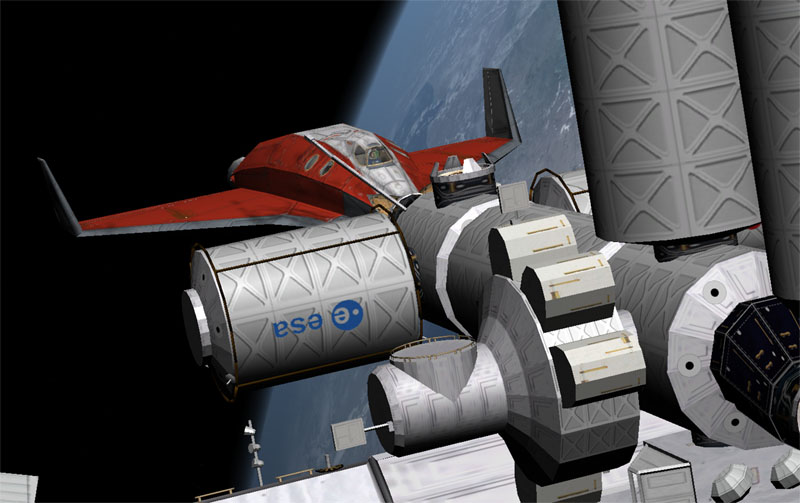
\includegraphics[width=0.75\hsize]{challenge_1.jpg}
	\caption{Checklist mission 1 completed successfully.}
\end{figure}


\subsection{Checklist mission 2: ISS to Mir transfer}
This mission consists of an orbital transfer from the International Space Station to the Russian Mir station (which in Orbiter's virtual reality is still happily orbiting Earth). Note that in Orbiter, Mir is placed in an ecliptic orbit to make it a platform for interplanetary missions. This means that ISS and Mir have a very high relative inclination which makes the transfer expensive in terms of fuel expenditure.

\begin{itemize}
\item Launch Orbiter with the \textit{Checklists/ISS to Mir} scenario. The mission starts with your glider docked at the ISS.
\item Press \keystroke{F1} to jump into the glider's cockpit.
\item Select target Mir in the Orbit MFD: Press Right-\Shift\keystroke{T}, \Enter, "mir".
\item To prepare for the high inclination orbit change, select the \textit{Align plane} mode in the left MFD: Left-\Shift\keystroke{F1}+\Shift\keystroke{A}, followed by \Shift\keystroke{T}+\Enter, "mir".
\item Undock from the ISS (\Ctrl\keystroke{D}). Once clear of the dock, close the nose cone (\keystroke{K}).
\item Switch to Orbit HUD mode (\keystroke{H}).
\item The first burn will take place at the DN (descending node) point. Use time compression to fast-forward there, but switch back to real-time when the "time-to-node" (TtN) value in the \textit{Align planes} MFD is down to 500.
\item Rotate the ship to the correct attitude for the burn: Click the \textit{Orbit-normal} (NML+) button. Wait until the glider has oriented itself perpendicular to the orbital plane (90° on the orbit inclination ladder).
\item When the \textit{time-to-burn} (TtB) counter for DN in the MFD display has counted down to 0, the [BURN] indicator will appear. Engage full main engines. The relative orbit inclination (RInc) should start to drop. Kill engines when the relative inclination reaches a minimum and the burn indicator disappears.
\item This is a very long burn (about 900 s), so you may want to fast-forward, but do not miss the end of the burn!
\item You probably won't be able to sufficiently reduce the relative inclination (to less than $\sim$0.5°) in a single burn. Repeat the process at the next node passage (at AN, ascending node). Remember that the glider must be oriented in the opposite direction for this burn, by activating the \textit{orbit-antinormal} (NML-) attitude function.
\item Once the orbital planes are sufficiently aligned, you need to plot a rendezvous trajectory using the \textit{Sync Orbit} MFD mode. The procedure is the same as in the previous mission.
\item Tune your NAV1 receiver to Mir's transponder frequency of 132.10 MHz, and NAV2 to the IDS frequency of docking port 1 at 135.00 MHz.
\item When the sync manoeuvre is complete, switch one of the MFD instruments to \textit{Docking} mode (\Shift\keystroke{F1}+\Shift\keystroke{D}) and make sure that NAV1 is selected for data input. Copy the setting to the HUD (\Shift\keystroke{H}).
\item Proceed with the docking manoeuvre to Mir in the same way as the ISS approach in the previous mission. Do not forget to open the nose cone before making contact.
\end{itemize}

\begin{figure}[H]
	\centering
	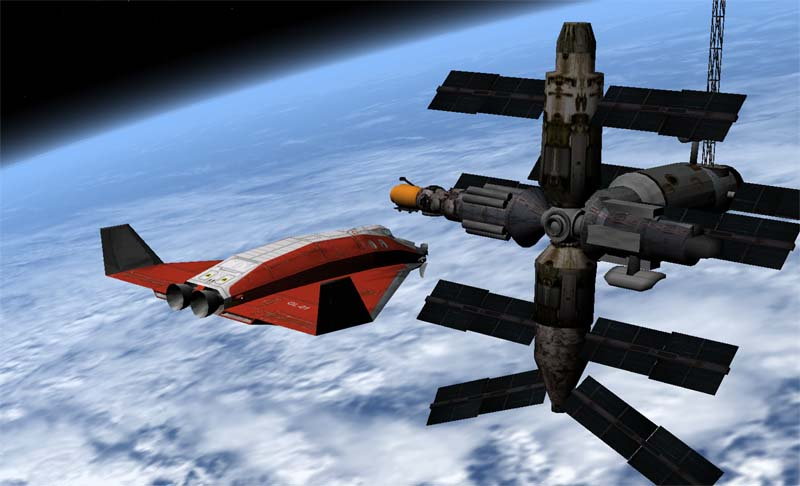
\includegraphics[width=0.75\hsize]{challenge_2.jpg}
	\caption{Docking approach to Mir space station.}
\end{figure}

\noindent
\textbf{Advanced version:} The long burn required for the plane change in this mission used up a lot of fuel. Try to find a more efficient way to perform this manoeuvre. Hint: The rotation of the orbital plane requires less Delta-V if the orbital velocity is lower. Can you perform an in-plane orbit change that will bring down the velocity to set up the plane rotation (and still requires less Delta-V in total than the direct rotation)?


\subsection{Checklist mission 3: De-orbit from Mir}
This mission completes your orbital round trip with a re-entry to return to Kennedy Space Center.

\begin{itemize}
\item Launch Orbiter with the \textit{Checklists/Deorbit} scenario. This picks up where the previous mission ended, with the glider docked to the Mir station. You are currently over the Pacific ocean, already in the correct location for the de-orbit burn.
\item Undock (\Ctrl\keystroke{D}) and wait for sufficient clearance from the station. You can use your retro engines (\keystroke{-}$_{Num}$) to increase separation velocity after reaching a safe distance.
\item Close the nose cone (\keystroke{K}).
\item Turn retrograde (\keystroke{]}).
\item When the glider’s attitude has stabilised and the retrograde direction is no longer obstructed by the station, engage main engines at 100\% thrust.
\item Cut engines when the perigee radius (PeR in Orbit MFD) has decreased to 5.600M.
\item Turn prograde (\keystroke{[}).
\item When attitude has stabilised, roll the glider level with the horizon (\keystroke{L}).
\item Switch to \textit{Surface} HUD mode (\keystroke{H}).
\item Switch the left MFD instrument to \textit{Surface} mode (\Shift\keystroke{F1}+\Shift\keystroke{D}).
\item You should reach 100 km altitude about 4000 km from the target (Dst: 4000M in the bottom line of the Map MFD). At this stage, aerodynamic forces will become noticeable.
\item At 50 km altitude, turn off attitude stabilisation (\keystroke{L}), disable the RCS (\keystroke{/}$_{Num}$) and make sure that attitude commands are routed to airfoils (AF CTRL dial is set to ON).
\item Lift forces now cause the glider to pitch up. To bleed off kinetic energy, perform left and right banks and pull the stick to put the glider into a high-AOA attitude. Due to the relatively high lift/drag ratio of the glider you need very steep bank angles (90°) to avoid reducing your descent rate in these manoeuvres.
\item The bank manoeuvres can also be used to increase the cross-range of your flight path. Your initial trajectory passes south of the KSC, so use left bank to correct the approach path (check Map MFD).
\item The bank angle determines your rate of descent and airspeed. If you come up short of the target, reduce the bank angle to slow your descent and reduce atmospheric deceleration. If you come in too fast or too high, increase the bank angles to increase the descent slope and atmospheric friction.
\item Timing of the reentry path is not quite as critical as for the Space Shuttle, because the glider can use its engines for a powered approach.
\item When the distance to target drops below 500 km, tune your NAV1 receiver to frequency 112.70 (KSCX VOR) and NAV2 to frequency 134.20 (Rwy 33 ILS) using the NAV/COM MFD mode (\Shift\keystroke{F1}+\Shift\keystroke{C}).
\item Switch an MFD to \textit{Horizontal Situation Indicator} (HSI) mode (\Shift\keystroke{F1}+\Shift\keystroke{H}). Leave the left HSI dial feed on NAV1, and flip the right dial to NAV2 (\Shift\keystroke{F}+\Shift\keystroke{N}).
\item Use the left dial for initial approach to KSC. Once in range of the ILS transmitter, use the course deviation and glide slope indicators on the right dial to line up your approach path to SLF runway 33. The HSI dials work like standard aircraft instruments.
\item Deploy airbrakes as required (\keystroke{B} to deploy by 1/2 step, \Ctrl\keystroke{B} to retract by 1/2 step). Lower landing gear at airspeed < 300 m/s. Touchdown speed is 200 m/s.
\item After touchdown, deploy airbrakes fully (\keystroke{B}+\keystroke{B}). Use wheel brakes at ground speed < 100 m/s (\keystroke{.} and \keystroke{,} \textit{simultaneously}), until you come to a halt.
\item Welcome back to Earth, commander!
\end{itemize}

\begin{figure}[H]
	\centering
	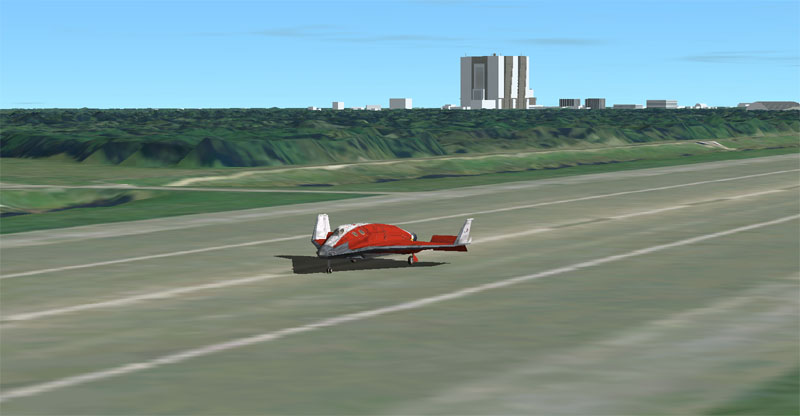
\includegraphics[width=0.75\hsize]{challenge_3.jpg}
	\caption{DG wheelstop at KSC SLF runway 33 after a successful return from orbit.}
\end{figure}


\subsection{Challenge missions}
The flight scenarios under the \textit{Challenges} folder put your flight skills to the test with missions that need to be completed with limited resources or by minimising fuel consumption. After completion of each mission, you get a score on how well the mission criteria were fulfilled. The available challenges are

\begin{itemize}
\item \textbf{Challenge 1: Launch and docking.} Launch the Delta-glider into orbit from the runway at Kennedy Space Center and dock with the ISS. Minimise fuel consumption (consider your launch window, launch azimuth, ascent profile, in-orbit manoeuvres). The score after completing the mission will reflect fuel expenditure.
\item \textbf{Challenge 2: Lunar transfer.} From low Earth orbit, perform a trans-lunar injection manoeuvre in your Delta-glider. On arriving at the Moon, enter a lunar orbit, and rendezvous and dock with the rotating wheel station. Again, the task is to minimise fuel consumption, so plan your engine burns carefully.
\item \textbf{Challenge 3: Advanced lunar transfer.} This is similar to the previous challenge, but this time you start out-of-plane of the Moon’s orbit, so you will have to consider an initial plane alignment, or an out-of-plane lunar transfer. The latter is trickier to plan, but may save on Delta-V, resulting in a higher score.
\item \textbf{Challenge 4: Entry and landing.} This scenario starts in a high Earth orbit. The objective is to de-orbit and land at Kennedy Space Center. The problem: your main and RCS fuel levels are very low, and you are not allowed to refuel during the mission. Plan your de-orbit burn and descent profile carefully! If the landing succeeds, the score rewards any fuel left over.
\end{itemize}


\end{document}
